% !TEX root = ../notes_template.tex
\chapter{Renal Filtration, Reabsorption \& Secretion}\label{chp:blood_content}
Updated on \today
\minitoc

This chapter covers the concept of mass balance with a particular focus on water and electrolyte mass balance. The mass balance of water and electrolytes are supported by renal filtration, reabsorption and secretion. Water and electrolyte mass balance are importance processes in the support of plasma (and therefore blood) volume and the concentration of electrolytes in the extra-cellular fluid. In Chapter \ref{chp:ecf_microcirculation} it was clear that alterations in the plasma volume and concentration become transferred to the interstitial fluid and from there to the ICF. The regulation of body fluid volume and composition is accomplished by acting directly on the plasma. The kidneys (and other systems such as the gastrointestinal, metabolic, and pulmonary) participate in the regulation of the body fluid volume and composition by acting on the plasma.


\vspace{5mm}

\textbf{Objectives include:}
\begin{enumerate}
    \item
    \item
    \item
    \item
    \item
\end{enumerate}

\section{Mass Balance}

This chapter is the first to specifically discuss the concept of mass balance. Mass balance applies the conservation of mass and energy to the analysis of physical systems. It considers the mass and energy entering (inputs) and leaving a system (outputs). For the physical therapist the need for inputs into the human system is one reason for human function. To use the terms from the ICF model introduced in the Introduction, the inputs of food, drink and air require activity and participation (function). Many activities of daily living (ADLs) are based on the functional activities that provide appropriate inputs, and hygienic outputs required for physiological mass balance.

The inputs of food, drink and air ultimately provide the water, nutrients (macronutrients and micronutrients) and oxygen that are utilized for physiological processes. An overview of physiological mass balance is provided in Figure \ref{fig:mass_balance}. How these are used, whether they can be recycled, and the ways in which they are lost influences the time scale of the need for inputs. When describing outputs the term incidental loss refers to loss that occurs without purpose. Incidental loss is contrasted with intentional loss. An example of incidental loss is the loss of Na++ in sweat. The loss of water with sweat is purposeful as part of thermoregulation. But the loss of Na++ with sweat is unnecessary for the primary purpose of thermoregulation, but still requires replacement of Na++. Loss due to use such as oxygen in ETC, or due to a role being played in excretion of waste products such as water in feces and urine, is intentional loss. 

\begin{figure}[!h]
    \centering
    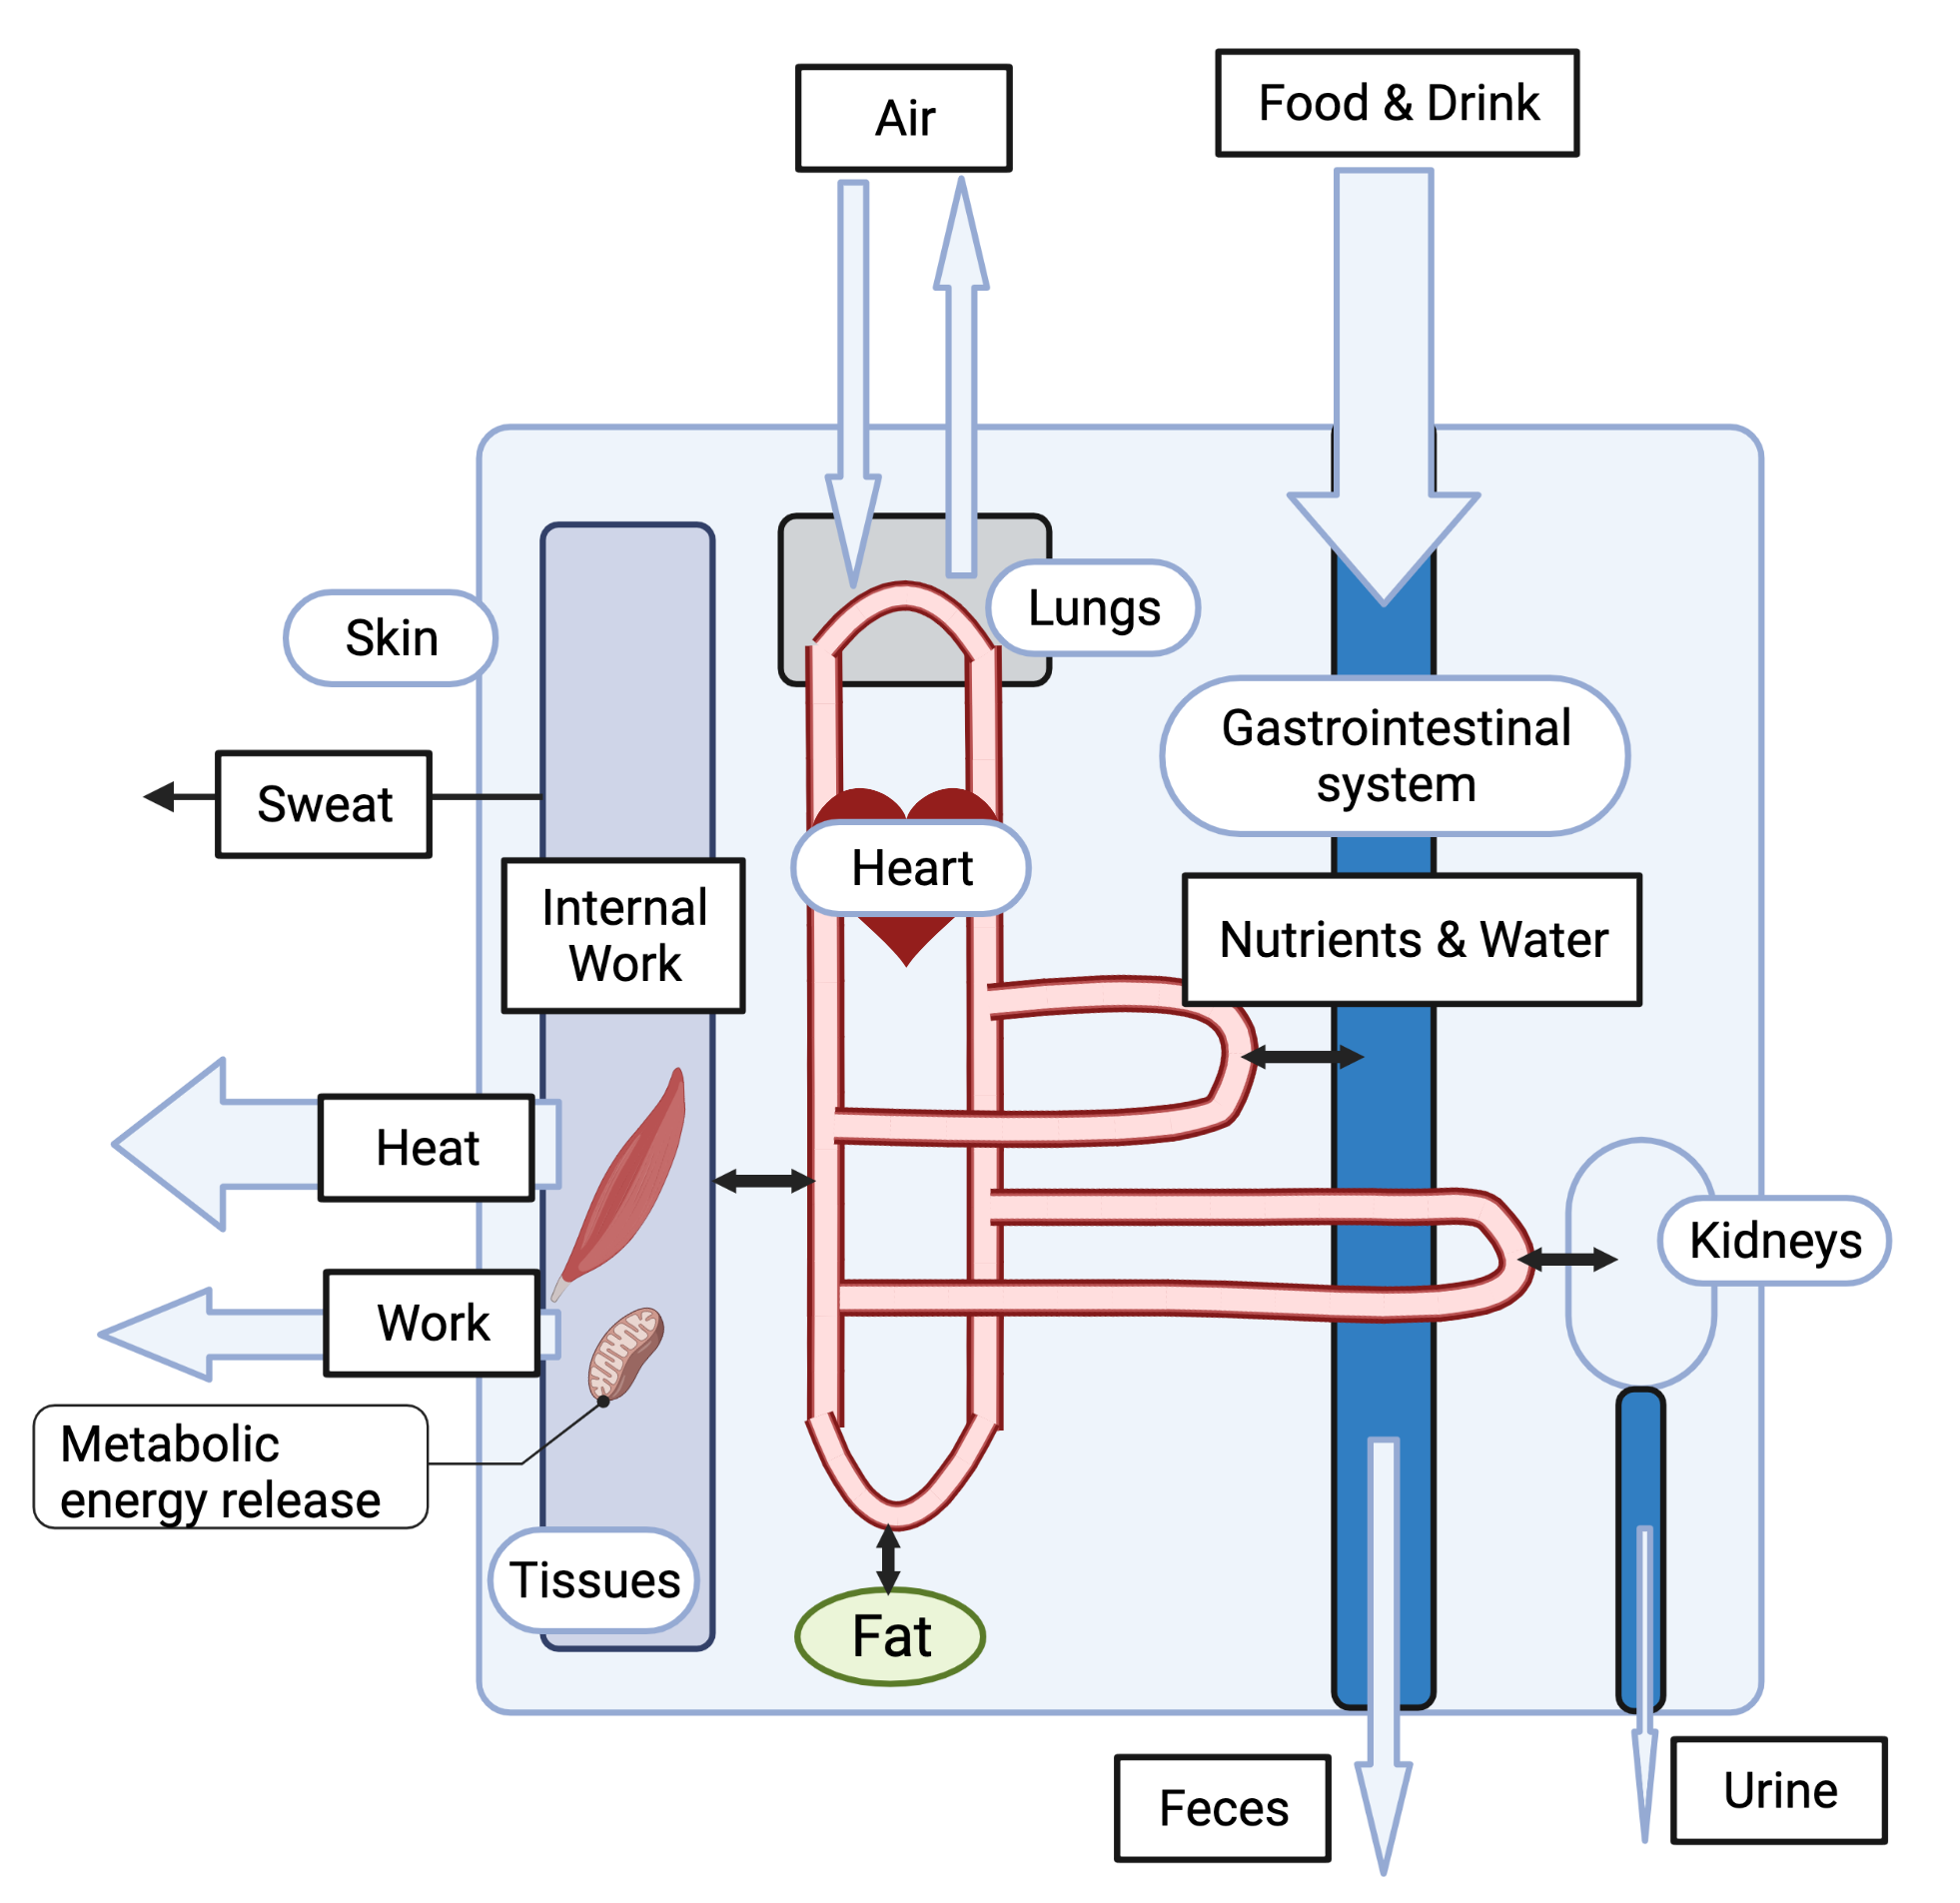
\includegraphics[width=1\linewidth]{./figure/mass_balance.png}
    \caption{Physiological Mass Balance \footnotesize{(Created with BioRender.com)}}
    \label{fig:mass_balance}
\end{figure}

\subsection{Oxygen Mass Balance}
Oxygen is used regularly and relatively quickly with very little storage (myoglobin) and no recycling, making the input of air with oxygen a regular requirement. Life is not sustainable for prolonged periods without the input of air over the time scale of a few minutes in most individuals. At nearly the same rate, and at times at a slightly higher rate, of oxygen utilization carbon dioxide is produced as a waste product of mitochondrial respiration. Input and output of air allows for both the input of oxygen, and the output of carbon dioxide. Oxygen and carbon dioxide mass balance is covered in Chapters \ref{chp:blood_oxygen} and \ref{chp:alveolar_oxygen}.


\subsection{Nutrient Mass Balance}

When discussing mass balance of nutrients, which includes the consideration of diet and nutrition since it is about the input of nutrients, it is common to break nutrients into two main classifications. Macronutrients are larger molecules that can be utilized for energy purposes (they have an energetic, that is caloric) value in addition to other physiological roles they fulfill. Macronutrients include carbohydrate, fat and protein. Micronutrients are small molecules and in some cases simply elements or minerals. They do not have an energetic (caloric) value but are essential to many physiological processes. For muscle physiology it has already become clear that Na+, K+ and Ca++ are essential micronutrients. Up to this point micronutrients (dietary inputs) have been considered in their physiological roles. Electrolytes when considering the role they have in determining the osmolarity of a solution; ions when considering the role they have in membrane potentials; and molecules when considering the role they play in activation (Ca++).

Macronutrients are routinely utilized for energy and system integrity (structural health of molecules such as hormones and neurotransmitters; as well as cellular structures, cells and tissues). However they are also stored purposely (fat is stored most abundantly as adipose tissue, carbohydrate as glycogen) or are available for extreme situations (protein is available for extreme situations from skeletal muscle). Proteins can be, at least partially, recycled. If a protein is broken down into amino acids and used to build an enzyme that is needed; it could be again broken down and used to build another enzyme. Similarly fat and carbohydrate utilized in structures can be recycled. However, macronutrients utilized for energy lose their structure and cannot be recycled, they must be replaced. The digestion of food to extract and absorb usable macronutrients\footnotemark\footnotetext{Once macronutrients are absorbed as carbohydrate or fat they are often referred to as substrates.} ultimately yields waste that remains in the gastrointestinal (GI) tract (for example, insoluble fiber) and is removed as feces. 

The lining of the GI tract not only absorbs all nutrients (macro and micro), but there is some incidental loss of micro-nutrients (electrolytes and minerals) such as Ca++ in the feces from the GI secretions and normal wear and tear of the cells and tissue that line the GI tract. A small amount of incidental loss of micronutrients such as Na+ and K+ occurs in the sweat and urine. Since the input of input of these micronutrients can easily exceed the incidental loss, there can be intentional (regulated) loss through the renal filtration, reabsorption and secretion processes to maintain Na+, K+ and Ca++ homeostasis.

Macronutrient mass balance is covered in Chapter \ref{chp:blood_nutrients}.

\subsection{Water Mass Balance}

Water is the source of the fluid environment from which the biochemical processes of life occur, and from which transport of essential nutrients flow through the circulation and micro-circulation Without water blood plasma, interstitial fluid and intra-cellular fluid would not be fluid. The fact that they are fluid enables nutrient movement. The amount of water in the body also influences the concentration (and therefore osmolarity) of these fluid spaces. The amount of water influences the blood volume. If too high blood pressure increases and edema may result. When too low viscosity increases which increases resistance to circulation. Problems occur when there is too little water (dehydration) or too much water (elevated blood volume, edema). The water in the body is always in use, being filtered between compartments in support of the movement of nutrients and electrolytes as well as by-products (waste). In this way it is recycled - there is no need for a complete overturn of water in the course of a day. However, the amount of water that must be taken in (input) should equal the amount of water that is lost in a day (output). Water loss occurs through four routes, two incidental and two intentional. Incidental water loss occurs with ventilation of air out of the body; and a small amount of water is routinely lost in the feces (it could be argued that water loss with feces (stool) is intentional to avoid hard difficult to pass stool. Evaporation of water from the skin is a mechanism of cooling the body and sweating is a route of loss. Intentional loss of water in sweat is highly variable based on the temperature and activity levels which influence the need for cooling. Renal filtration and excretion requires a loss of water in urine for the removal of metabolic waste. Of these four routes for the output of water sweating is highly variable and can be partially regulated through behavioral adaptations; renal is also highly variable and is regulated through physiological processes. The maintenance of normal water volume, and as a result plasma volume, is buffered by fluctuations in renal output in response to water input. Because there is a continual regular loss of water (breathing and sweating), and a necessary regular loss of water for waste removal (feces and urine), there is a regular need (demand) for water input. While the kidneys can make more or less concentrated urine which includes less or more water (respectively), the body must make urine regularly to filter the blood and keep it free from the toxicity of metabolic waste products.

Given the central role of renal filtration, reabsorption and secretion, and urinary excretion on plasma volume and content through water and micronutrient mass balance these topics are covered in this chapter.

\section{Renal Function}

Renal function relies on the kidneys. The kidneys have several important physiological functions. 

\begin{enumerate}
    \item Excretion: The kidneys ensure that harmful substances are excreted in urine. Harmful substances can be absolutely harmful (waste products such as urea), or relatively harmful (electrolytes when they exceed their normal ranges).
    \item Regulation \& Buffer: The kidneys regulate and therefore buffer the mass balance of plasma, and therefore body, water and electrolyte amounts and therefore through both water and the electrolyte amount they regulate electrolyte concentrations (micro-circulation support).
    \item Regulation: Through the regulation of plasma volume the kidneys provide long term regulation to blood pressure (circulation support).
    \item Endocrine: The kidneys synthesize and secrete three hormones: renin for the regulation of blood pressure; erythropoietin for the regulation of red blood cells; and 1,25-dihydroxycholecalciferol for the regulation of Ca++.
\end{enumerate}

Functions 1, 2 and 3 and the endocrine function of renin are covered in this chapter. The endocrine function of erythropoietin is covered in the Chapter \ref{chp:blood_oxygen} on Respiration; and of 1,25-dihydroxycholecalciferol in Chapter \ref{chp:blood_nutrients} on Digestion-Absorption-Metabolism.

\section{Functional Anatomy}


\section{Urine Formation \& Excretion}

 overall function of the renal system is to regulate the volume and composition of body fluids. The body fluids consist of three major compartments: the ICF, the ISF, and the plasma. In a normal young adult male, these comprise about 40\%, 15\%, and 5\% of body weight, respectively. These volumes can be calculated from the volume of distribution of marker substances that distribute themselves according to the TBW, ECF, or the plasma. The intracellular volume is the TBW minus the ECF; the ISF volume is calculated as the ECF minus the plasma. The volumes of the various fluid compartments vary with age, gender, and body composition. Fat tissue has little water, so excess body fat contributes excess body weight without much added water. Therefore, using the idea of an LBM containing 73\% water, it is possible to estimate excess body fat from body weight and TBW. The presence of anionic proteins in the plasma which cannot equilibrate across the capillary wall sets up a slightly unequal concentration of diffusible ions across the capillary. This is due to the Gibbs–Donnan effect, which produces a negative potential on the side of the impermeant anion. The potential can be calculated from the Nernst equation. The body fluids reside in well-defined anatomic compartments, and there are barriers and forces that determine exchange between the compartments. The distribution of electrolytes and water can be visualized using Darrow–Yannet diagrams. In these calculations, we assume that water equilibrates its osmotic pressure across all boundaries, Na+ remains extracellular, and K+ remains intracellular. From this analysis, we can see that ingestion of water expands ICF and ECF compartments while diluting their osmolarity; ingesting NaCl alone expands the ECF and concentrates both ECF and ICF solutes; ingestion or infusion of isotonic saline expands only the ECF with no changes in ICF.

The renal system accomplishes its task of regulating body fluid compartment size and composition by operating solely on the plasma. Changes in plasma fluid volume and composition are then transferred to the ISF and ICF. Other organ systems also participate in this regulation.

\subsection{Glomerular Filtration}

\subsection{Tubular Reabsorption \& Secretion}

\subsection{Urine Concentration \& Dilution}

\subsection{Micturation}

\section{Renal Regulation}

\subsection{Blood Volume}

\subsection{Osmolarity}

\subsection{Micronutrients}




\section{\textit{Muscle Connections}}

\subsection{Dehydration}

\subsection{Rhabdomyolosis}

\subsection{Urinary Incontinence}

\section{Uromysotisis Poisoning}

A fictional condition created by Jerry Seinfeld and Larry David to justify Jerry's need to urinate in a mall parking garage when he and his friends lost their car and had to wander the garage for hours (See \href{https://www.youtube.com/watch?v=OG6b7KJ1Ah0}{Seinfeld-Parking Garage}). Uromysotisis poisoning is a potentially deadly condition resulting from holding in one's urine for a prolonged period of time. The condition can result in acute poisoning when one is restricted by the arbitrary rules of society. Common treatments for uromysotisis include the "pee party".

\section{Summary}

\subsection{Next Step}

\printbibliography[heading=subbibintoc]